\section{Design of UPRESSO}
\label{sec:UPRESSO}
In this section, we provide designs of UPRESSO, a secure and privacy-preserving SSO system.
First, we present how to achieve the trapdoor user identification and transformed receiver designation. Then, we describe the detailed protocol for providing the SSO service. Finally, we discuss the compatibility of UPRESSO with OIDC.

\subsection{Features}
\label{subsec:overview}
The three functions $F_{PID_{RP}}$, $F_{PID_U}$ and $F_{Account}$  are essential for the trapdoor user identification and  transformed receiver designation.
In UPRESSO, these functions are constructed based on discrete logarithm cryptography with the public parameters $p$, $q$ and $g$,
 where  $p$ is a large prime defines the finite field $GF(p)$,  the prime number $q$  is the order of a multiplicative
subgroup of $GF(p)$, which is generated with the generator $g$ by $\{g\ mod\ p, g^2\ mod\ p, ..., g^{q-1}\ mod\ p, 1=g^q\ mod\ p\}$.

In UPRESSO, IdP assigns a  random number as  $ID_U$ ($0 < ID_U <q $)  at the user's registration, and chooses a random number $r$ ($1 < r < q$) to generate $ID_{RP}$ at the RP's initial registration. The $r$ must  be different from the ones chosen before, and $ID_{RP}$ is generated using Equation~\ref{equ:IDRP}.
   \begin{equation}
   ID_{RP} = g^{r} mod \ p
   \label{equ:IDRP}
   \end{equation}

For each login, the RP chooses a random number $n_{RP}$ ($1 < n_{RP}<q $), the user chooses a random number $n_{U}$ ($1 < n_{U}<q $). Then, the RP and user cooperatively  generate $PID_{RP}$ using the function $F_{PID_{RP}}$ as Equation~\ref{equ:PIDRP}. The function $F_{PID_{RP}}$ satisfies the requirements described in Section~\ref{subsec:challenges}. That is, the function $F_{PID_{RP}}$ is invoked to generate $PID_{RP}$ for each login, while IdP  fails to derive $ID_{RP}$ from $PID_{RP}$ and cannot find the relation among ${PID_{RP}}$s for a same RP, which is ensured by the discrete logarithm cryptography.
Moreover, $n_{U}$ and $n_{RP}$  serves as the nonce which ensures that the $PID_{RP}$ (also identity proof) is exactly constructed for this login, and
the cooperation between the user and RP prevents the malicious user and RP from controlling the  $PID_{RP}$. For example, the malicious user fails to make a correct RP accept a $PID_{RP}$ used in another login, while the collusive RPs fail to use a same or correlated $PID_{RP}$s for different logins.


 \begin{equation}
    PID_{RP} = {ID_{RP}}^{n_{u}* n_{RP}} mod \ p
   \label{equ:PIDRP}
   \end{equation}

For the user $ID_U$ to login at an RP with a privacy-preserving identifer $PID_{RP}$, IdP calculates the user's privacy-preserving identifer $PID_U$ using the function  $F_{PID_{U}}$ as Equation~\ref{equ:PIDU}. The function $F_{PID_{U}}$ satisfies the requirements described in Section~\ref{subsec:challenges}. 
Combining Equation~\ref{equ:IDRP},~\ref{equ:PIDRP} and~\ref{equ:PIDU}, we get that  $PID_U$ equals to $g^{r*n_U*n_{RP}*ID_U}\ mod \ p$.
The discrete logarithm cryptography ensures that the RPs fail to derive $ID_U$ from $PID_U$,
nor link a user's $PID_U$s at different RPs who do not know $r$ and $ID_U$.

   
\begin{equation}
 PID_U = {PID_{RP}}^{ID_U} \ mod \ p
 \label{equ:PIDU}
\end{equation}

Finally, the RP derives $Account$ for the user with the function $F_{Account}$ as Equation~\ref{equ:Account}. Here, the value $(n_U*n_{RP})^{-1} mod \ q$ is the trapdoor $t$. As $q$ is a prime number, $1< n_U < q$ and $1< n_{RP} < q$, therefore $q$ is coprime to $n_U*n_{RP}$, and the $t$ that satisfies $t*(n_U*n_{RP}) = 1\ mod \ q$ always exists. The function $F_{Account}$ satisfies the requirements described in Section~\ref{subsec:challenges}.  As shown in Equation~\ref{equ:AccountNotChanged},  $F_{Account}$ outputs an unchanged $Acount$ for a user's multiple logins at an RP. 
Combining Equation~\ref{equ:IDRP},~\ref{equ:PIDRP}, ~\ref{equ:PIDU} and~\ref{equ:AccountNotChanged}, we get that $Account$ equals to $g^{r*ID_U} mod \ p$.
Same as the analysis of $PID_U$s, the collusive RPs fail to derive $ID_U$ from $Account$ nor link a user's $Account$s at different RPs without knowing $r$ and $ID_U$.

 \begin{equation}
   Account = {PID_U}^{(n_U*n_{RP})^{-1} mod \ q} mod \ p
   \label{equ:Account}
   \end{equation}

The \textbf{trapdoor user identification} is supported with these three functions.
For a user's multiple logins, each PR obtains the different $PID_U$s and the corresponding $t$s , then derives the unchanged $Account$  as shown in Equation~\ref{equ:AccountNotChanged}.
The function $F_{PID_{RP}}$ prevents the curious IdP from linking the $PID_{RP}$s of different logins at an RP, and therefore avoids  the  IdP-based access tracing.
The functions $F_{PID_{U}}$ and $F_{Account}$ prevents the collusive RPs from linking a user's $PID_U$s and $Account$s at different RPs, and therefore avoids the RP-based identity linkage.
 \begin{multline}\label{equ:AccountNotChanged}
   Account =  {PID_{U}}^{t} mod \ p  \\
   = {({PID_{RP}}^{ID_U})}^{{(n_U*n_{RP})^{-1} mod \ q}} mod \ p \\
   = {ID_{RP}} ^ {ID_U * n_U * n_{RP} *t\ mod\ q} = {ID_{RP}}^{ID_U} mod \ p
 \end{multline}

The \textbf{transformed receiver designation} is also supported with the efficient functions $F_{PID_{RP}}$ and $F_{PID_U}$, together with  a user-centric verification.
The $F_{PID_{RP}}$ ensures that the user and RP cooperatively generate a fresh $PID_{RP}$  for a user's login,
 while $F_{PID_U}$ ensures that the IdP generates the exact $PID_U$ for the $ID_U$ who logins at $PID_{RP}$.
The IdP will bind $PID_{U}$ with $PID_{RP}$ in the identity proof, which designates this identity proof to $PID_{RP}$.
In the user-centric verification,  the user checks that $PID_{RP}$ is global unique and exactly generated for the RP $ID_{RP}$,
 and then sends the identity proof  only  to this RP. Therefore, the $PID_{RP}$ is designated to $ID_{RP}$.
Finally, the transformed receiver designation is provided through the two-step designations.


\begin{table*}[tb]
    \caption{The notations used in UPRESSO.}
    \centering
    \begin{tabular}{|c|c|c|}
    \hline
    {Notation} & {Definition} & {Attribute} \\
    \hline
    {$p$} & {A large prime.} & {System-unique} \\
    \hline
    {$g$} & {A primitive root  modulo $p$. } & {System-unique} \\
   % \hline
    %{$SK_{ID}$, $PK$} & {The private/public key to sign/verify identity proof.} & {System-unique} \\
    \hline
    {$ID_U$} & {User's unique identifier at IdP.} & {System-unique} \\
    \hline
    {$PID_U$} & {User's privacy-preserving id in the identity proof.} & {One-time}\\
    \hline
    {$Account$} & {User's identifier at an RP.} & {RP-unique} \\
    \hline
    {$ID_{RP}$} & {RP's original identifier.} & {System-unique} \\
    \hline
    {$PID_{RP}$} & {The privacy-preserving $ID_{RP}$ transformation.} & {One-time} \\
    \hline
    {$n_U$} & {User-generated random nonce for $PID_{RP}$.} & {One-time} \\
    \hline
    {$n_{RP}$} & {RP-generated random nonce for $PID_{RP}$.} & {One-time} \\
    \hline
    {$Y_{RP}$} & {Public value for $n_{RP}$, $(ID_{RP})^{n_{RP}} \ mod p$.} & {One-time} \\
    \hline
    {$t$} & {A trapdoor, $t=(n_U*n_{RP})^{-1} mod \ (p-1)$.} & {One-time} \\
    \hline
    {$Cert_{RP}$} & {An RP certificate. } & {System-unique} \\
    \hline
    {$SK$, $PK$} & {The private/public key of IdP. } & {System-unique} \\
     \hline
    \end{tabular}
    \label{tbl:notations}
\end{table*}

\subsection{The implementations of UPRESSO}
\label{implementations}
To lead the forementioned features be implemented in UPRESSO, it requires the system initialization is performed to initialize the IdP only once at the very beginning of system construction and generates key parameters for further initiation and login process. Moreover, the RP should be initiated before it attaches the UPRESSO system, when the IdP provides the $ID_{RP}$ and unforgeable RP proof (denoted as $Cert_{RP}$). Next, we will describe the System initialization, RP initial registration and the algorithms for calculating  $PID_{RP}$, $PID_U$ and $Account$.

\vspace{1mm}\noindent \textbf{System initialization.} The IdP generates the random asymmetric key pair, ($SK, PK$),
for calculating the signatures in the identity proof and $Cert_{RP}$, respectively;
and provides $PK$ and $PK$ as the public parameters for the verification of identity proof and $Cert_{RP}$.
Moreover, IdP generates a strong prime $p$, calculates  a primitive root ($g$), and provides $p$ and $g$ as the public parameters.
For $p$, we firstly randomly choose a large prime $q$, and accept  $2q+1$ as $p$ if $2q+1$ is a prime.
The strong prime $p$ makes it easier to choose $n_{u}$ and $n_{RP}$ at the user and RP for the RP identifier transformation (detailed in  Section~\ref{subsec:identifier-generation}). %With $g$, we obtain all the integers less than $p$, by calculating $g^i mod \ P$ for $0 \leq i \leq (P-1)$.
Once $SK$ leaked, IdP may update this asymmetric key pair.
However, $g$ and $p$ will never be modified, otherwise, the RPs fail to link the user's accounts between two different $p$ (or $g$).
%The IdP setup and following RP initial registration are based on the features of primitive root.


\vspace{1mm}\noindent\textbf{RP initial registration.}
The RP invokes an initial registration to apply a valid and self-verifying $Cert_{RP}$ from IdP (\textbf{Goal 1}),
% as provided in Figure~\ref{fig:registration}
 which contains three steps:

\begin{enumerate}
\item RP sends IdP a $Cert_{RP}$ request $Req_{Cert_{RP}}$, which contains the distinguished name $Name_{RP}$ (e.g., DNS name) and the endpoint to receive the identity proof.
\item IdP calculates $ID_{RP} = g^r mod \ p$ with a random chosen $r$ which is coprime to $p-1$ and different from the ones for other RPs,  generates the signature ($Sig_{SK}$) of [$ID_{RP}, Name_{RP}$] with $SK$, and returns [$ID_{RP}, Name_{RP}, Sig_{SK}$] as $Cert_{RP}$.
\item IdP sends $Cert_{RP}$ to the RP who verifies $Cert_{RP}$ using $PK$.
\end{enumerate}



%1. r which is coprime to $P-1$来保证$ID_{RP}$是一个本原根,从而保证adversary无法从PID中获取ID_U, ---
%2. $ID_{RP}$不能相同,保证RP无法进行identity linkage。 ---RP可以借助类似CT的方案来保证, 没有两个合法证书被颁发给同一个ID_{RP}
To satisfy RP fails to derive $ID_U$ from $Account$ and the $Accounts$ of a user are different among RPs in \textbf{Goal 3}, two requirements on $r$ are needed  in $ID_{RP}$ generation:
\begin{itemize}
  \item $r$ should be coprime to $p-1$. This makes $ID_{RP}$ also be  a primitive root, and then prevents the RP from inferring $ID_U$ from $Account$, which is  ensured by the discrete logarithm problem.

  \item  $r$ should be different for different RPs. Otherwise, the RPs assigned the same $r$ (i.e., $ID_{RP}$), will derive the same $Account$ for a user, resulting in identity linkage. % possible.
\end{itemize}

\vspace{1mm}\noindent\textbf{Algorithms for calculating  $PID_{RP}$, $PID_U$ and $Account$.} Moreover, we provide the algorithms for calculating  $PID_{RP}$, $PID_U$ and $Account$,
which are the foundations to process each user's login.

\noindent\textbf{$PID_{RP}$}. Similar to Diffie-Hellman key exchange\cite{DiffieH76}, the RP and user negotiate the  $PID_{RP}$ as follows:
\begin{itemize}
  \item RP chooses a random odd number $n_{RP}$, and sends $Y_{RP} = {ID_{RP}}^{n_{RP}} mod \ p$ to the user.
  \item The user replies a random chosen odd number $n_{u}$ to the RP, and calculates $PID_{RP} = {Y_{RP}}^{n_{u}} mod \ p$.
  \item RP also derives $PID_{RP}$ with the received $n_{u}$.
\end{itemize}

As denoted in Equation~\ref{equ:RPIDT}, ${ID_{RP}}$ cannot be derived from $PID_{RP}$, which satisfies IdP never infers ${ID_{RP}}$ from $PID_{RP}$ in \textbf{Goal 2}.
   \begin{equation}
   PID_{RP} = {Y_{RP}}^{n_{u}} = {ID_{RP}}^{n_{u}* n_{RP}} mod \ p
   \label{equ:ID_{RP}T}
   \end{equation}

To ensure $PID_{RP}$ not controlled by the adversary in \textbf{Goal 2},
 $PID_{RP}$ should not be determined by  either the RP or user.
Otherwise, malicious users may make the victim RP accept an identity proof issued for another RP; or collusive RPs may provide the correlated $PID_{RP}$ for potential identity linkage.

In UPRESSO, RP fails to control the $PID_{RP}$ generation, as it provides $Y_{RP}$ before obtaining $n_{u}$ and the modification of $Y_{RP}$ will trigger the user to generate another different  $n_{u}$. The Discrete Logarithm problem prevents the user from choosing an $n_{u}$ for a specified $PID_{RP}$ on the received $Y_{RP}$.

In UPRESSO, both $n_{RP}$ and $n_{u}$ are odd numbers, therefore $n_{RP}*n_{u}$ is an odd number and coprime to the even $p-1$, which ensures that the inverse $(n_{RP}*n_{u})^{-1}$ always exists, where  $(n_{RP}*n_{u})^{-1} * (n_{RP}*n_{u}) = 1 \ mod \ (p-1)$. The inverse  serves as  the trapdoor $t$ for $Accout$, which makes:
\begin{equation}
(PID_{RP})^t = ID_{RP} \ mod \ p
\label{equ:trapdoor}
\end{equation}


\noindent\textbf{$PID_U$}. The IdP generates the $PID_U$ based on the user's $ID_U$ and the user-provided $PID_{RP}$, as denoted in Equation~\ref{equ:PID_U}.
The corporative generation of $PID_{RP}$, ensures unrelated $PID_U$  for different RPs in \textbf{Goal 3}. Also, RP fails to derive $ID_U$ from either $PID_U$ in \textbf{Goal 3}, as
   $PID_{RP}$ is a primite root modulo $p$, and the $ID_U$ cannot be derived from $PID_{RP}^{ID_U}$.
\begin{equation}
 PID_U = {PID_{RP}}^{ID_U} \ mod \ p
 \label{equ:PID_U}
\end{equation}

Finally, the RP calculates $(PID_U)^t mod \ p$ as the  user's account, where $PID_U$ is received from the user and $t$ is derived in the generation of $PID_{RP}$. Equation~\ref{equ:account} demonstrates that $Account$ is unchanged to the RP during a user's multiple logins, satisfying RP derives the user's unique $Account$  from $PID_U$ with the  trapdoor and  RP fails to derive $ID_U$ from either $Account$ in \textbf{Goal 3}. The different $ID_{RP}$ ensures the $Accounts$ of a user are different among RPs in \textbf{Goal 3}.

 \begin{equation}
   Account = (PID_U)^{(n_U*n_{RP})^(-1) mod \ q}
   \label{equ:account}
   \end{equation}


\subsection{Overall protocol flow overview}
\label{sebsec:loginprocess}
In this section, we present the detailed process for each user's login as shown in Figure~\ref{fig:process}.

\begin{figure*}
  \centering
  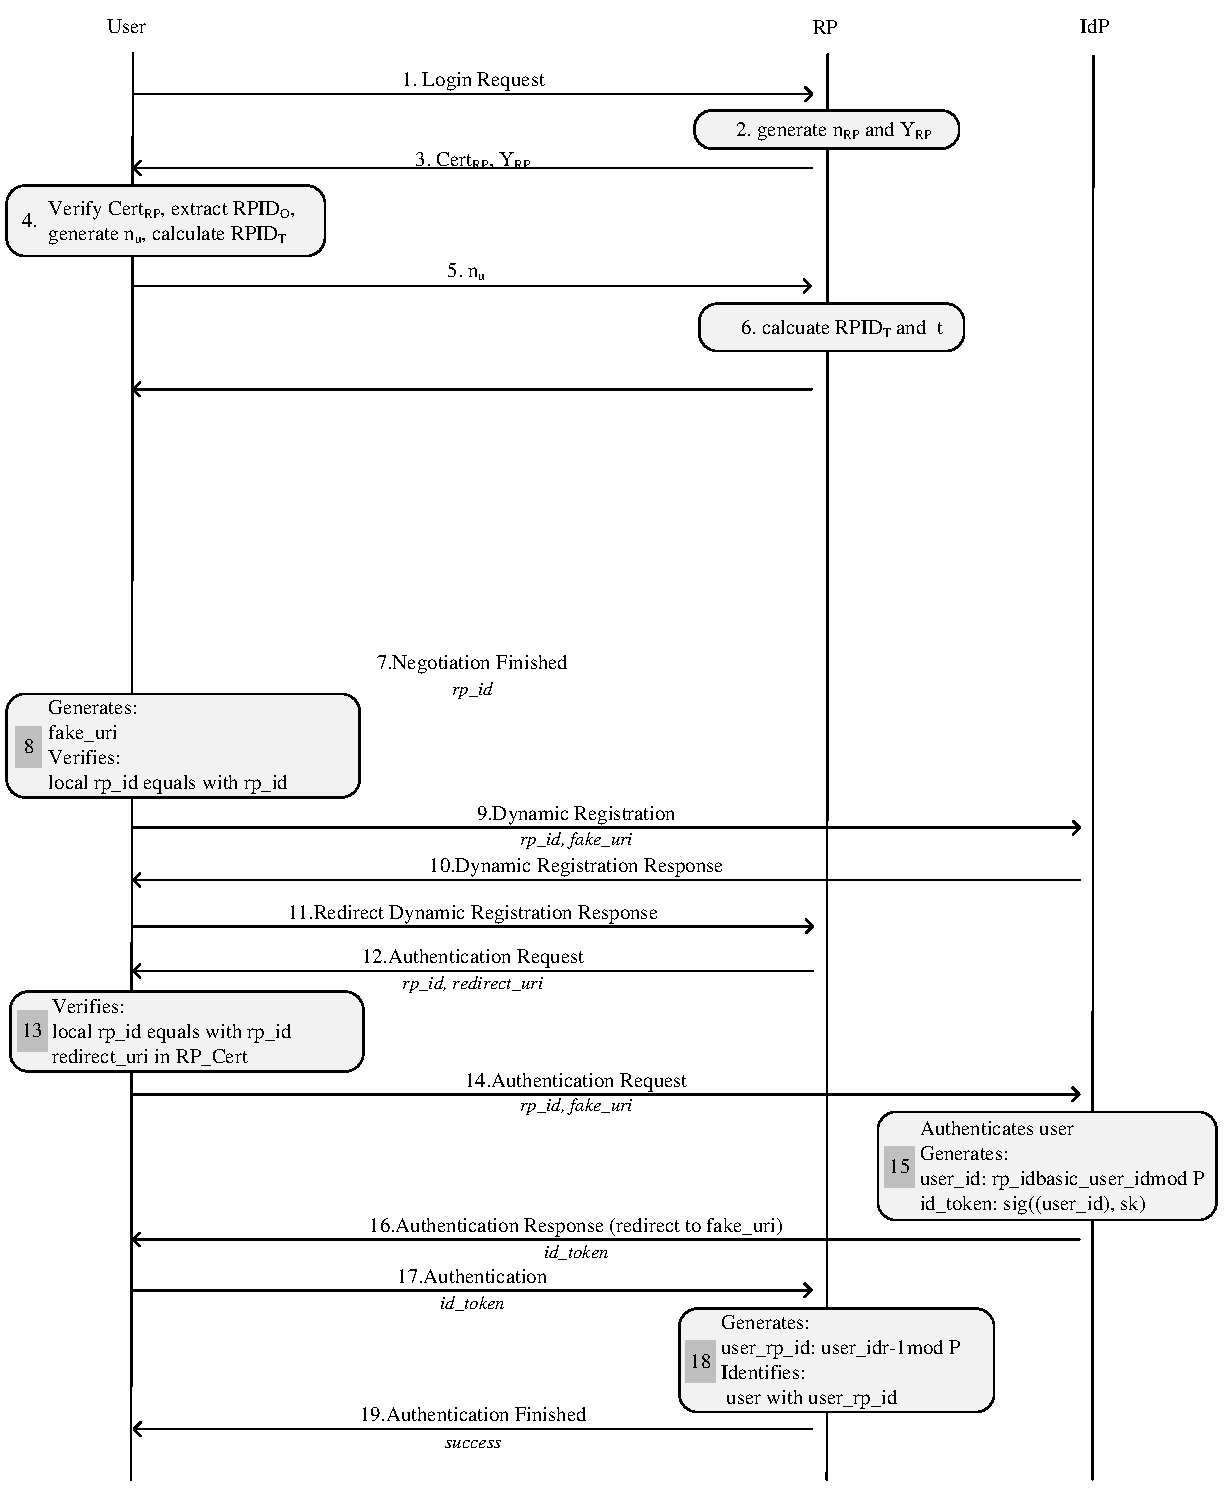
\includegraphics[width=0.85\linewidth]{fig/process.pdf}
  \caption{Process for each user login.}
  \label{fig:process}
\end{figure*}

In RP identifer transforming phase, the user and RP corporately process as follows. \textbf{(1)} The user sends a login request to trigger the negotiation of $PID_{RP}$. \textbf{(2.1.1)} RP chooses the random $n_{RP}$, and calculates $Y_{RP}$ as described in Section~\ref{subsec:identifier-generation}. \textbf{(2.1.2)} RP sends $Cert_{RP}$ with $Y_{RP}$ to the user.  \textbf{(2.1.3)} The user halts the login process if the provided $Cert_{RP}$ is invalid; otherwise, it extracts $ID_{RP}$ from $Cert_{RP}$, and calculates $PID_{RP}$ with a random chosen $n_U$ as in Section~\ref{subsec:identifier-generation}. \textbf{(2.1.4)} The user sends $n_U$ to the RP. \textbf{(2.1.5)} RP calculates $PID_{RP}$ using the received $n_U$ with $Y_{RP}$ as in Section~\ref{subsec:identifier-generation}. After that, RP derives the trapdoor $t$ as in Section~\ref{subsec:identifier-generation}, which will be used in calculating $Account$. \textbf{(2.1.6)} RP sends the calculated $PID_{RP}$ to the user, who will halt the login if the received $PID_{RP}$ is different from the cached one.

In the RP identifier renewal phase, the user registers the newly generated $PID_{RP}$ at the IdP as follows. \textbf{(2.2.1)} The user generates an one-time endpoint (used in Section~\ref{subsec:compatible}) if the received $PID_{RP}$ is accepted. \textbf{(2.2.2)} Then, the user registers the RP with the $PID_{RP}$ and one-time endpoint. \textbf{(2.2.3)} If $PID_{RP}$ is globally unique and is a primitive root module $p$, IdP sets the flag $RegRes$ as $OK$ (otherwise $FAIL$), and constructs the reply in the form of
[$RegRes$, $RegMes$, $Sig_{SK}$]
%[$RegRes$, $timestamp$, $PID_{RP}$, $Sig_{SK_ID}$] where $timestamp$ is the time generating this reply and
where $RegMes$ is the response to original dynamic registration containing $PID_{RP}$, issuing time as well as other attributes and $Sig_{SK}$ is the signature of the other elements using the private key $SK_{ID}$ (ensuring unique $PID_{RP}$ for binding in \textbf{Goal 2}). \textbf{(2.2.4)} The user forwards the registration result to the RP. The user obtains $RegRes$ directly as the connection between the user and IdP is secure, while the RP accepts the $RegRes$ only when $Sig_{SK}$ is valid
%, $timestamp$ is correct and $PID_{RP}$ is the same as the cached one.
and $RegMes$ is issued for the $PID_{RP}$ within the valid period. The user and RP will negotiate a new $PID_{RP}$ if $RegRes$ is $FAIL$.

To acquire the $PID_U$, the user corporates with the RP and IdP as follows. \textbf{(2.3)} RP constructs an identity proof request with the correctly registered $PID_{RP}$ and the endpoint (the form of the request is detailed in Section~\ref{subsec:compatible}). \textbf{(2.4)} The user halts the login process if the received $PID_{RP}$ is different from the previous one. \textbf{(2.5)} The user replaces the endpoint with the registered one-time endpoint, and sends it with the identity proof request to the IdP. \textbf{(3)} IdP requires the user to provide the correct credentials if the user hasn't been unauthenticated. \textbf{(4)} IdP rejects the request if the binding of $PID_{RP}$ and the one-time endpoint doesn't exist in the registered ones. Then, IdP generates the $PID_U$ as in Section~\ref{subsec:identifier-generation}, and constructs the identity proof with $PID_{RP}$, $PID_U$, the valid period, issuing time and other attribute values, by attaching a signature of these elements using the private key $SK$. \textbf{(5.1)} IdP sends the identity proof with the one-time endpoint to the user. \textbf{(5.2)} User agent replaces the one-time endpoint with the correct endpoint. \textbf{(5.3)} The user forwards the identity proof to the RP's endpoint corresponding to the one-time endpoint.

Finally, RP derives the user's  $Account$ from $PID_U$ as follows. \textbf{(6)} RP accepts the identity proof only when the signature is correctly verified with $PK$, $PID_{RP}$ is the same as the negotiated one, the issuing time is less than current time, and the current time is in the validity period. If the identity proof is incorrect, RP returns login fail to the user who will trigger another login request. Otherwise, RP calculates the $Account$ as in Section~\ref{subsec:identifier-generation}. \textbf{(7)} RP sends the login result to the user and begins to provide the personalized service.


\subsection{Compatibility with OIDC}
\label{subsec:compatible}
UPRESSO is compatible with the implicit protocol flow of OIDC (authorization code flow is discussed in Section~\ref{sec:discussion}).

\vspace{1mm}\noindent \textbf{Consistent with OIDC.}
The entities in UPRESSO are same as them in OIDC (e.g. IdP, RP and user), which means it is not needed to introduce new trusted parties into this system and able to make UPRESSO owns the similar process with OIDC. The RP identifier renewal, $PID_U$ generation and $Account$ acquiring phases are in line with the OIDC process.

In UPRESSO, the formats of identity proof request and identity proof are the same as the ones in OIDC. In details, each element of the identity proof request in OIDC is contained in UPRESSO as follows: the RP's identifier ($PID_{RP}$ in UPRESSO), the endpoint (one-time endpoint in the request from the user in UPRESSO) and the set of required attributes (also supported by UPRESSO but not listed here). The identity proof in UPRESSO is also exactly the same as the one in OIDC, which includes RP's identifer ($PID_{RP}$ in UPRESSO), the user's PPID ($PID_U$ in UPRESSO), the issuer, validity period, issuing time, other requested attributes and a signature generated by $SK_{IdP}$.

The same formats of identity proof request and identity proof make the verification same in OIDC and UPRESSO. The IdP, in both UPRESSO and OIDC, verifies the identity proof request, by checking whether the mapping of RP's identifier and endpoint exists in the registered ones. The RP, in both UPRESSO and OIDC, verifies the identity proof, by checking the signature, the consistency of RP's identifer in the identity proof and the one it owns, the validity period, issuing time and the freshness (which is checked based on a nonce in  OIDC, while  $PID_{RP}$ serves as the nonce in UPRESSO).

To avoid extra processes are added to UPRESSO compared with OIDC, the RP identifier renewal is implemented based on the dynamic registration (described in Section~\ref{sec:background}) provided by IdP in OIDC.

\vspace{1mm}\noindent \textbf{Minimal modification to OIDC.}
Although the process is same in UPRESSO and OIDC, there is also minimal modification in the values generating and parsing.

In UPRESSO, the dynamic registration in RP identifier renewal is invoked by the user instead of the RP to prevent the curious IdP linking the new registered RP identifier with specific RP.
As the registration response is transmitted through the user instead of server-to-server transmission between RP and IdP, the extra signature is required to guarantee the integrity of response.

In the $PID_U$ generation phase, compared with original $PPID$ picking in OIDC (IdP pick the corresponding $PPID$ from database based on the RP and user identifier), the $PID_U$ is temporarily calculated with current $PID_{RP}$ and $ID_U$ for each login instead of previously generated (for the first request) for all authentication requesting (expect for the first request).

In $Account$ acquiring phase, RP need the extra process to derive the user RP-uniquely identifier $Account$ from $PID_U$ which does not exist in OIDC as the $PPID$ is able take the same responsibility as $Account$.

\vspace{1mm}\noindent \textbf{Newly added features.}
Compared with OIDC, the RP identifier transforming phase is added in UPRESSO to build one-time temporary transformed RP identifier (e.g., $PID_{RP}$). The RP identifier transforming required the negotiation between RP and user to generated the random identifier based on RP's registered identifier (e.g., $ID_{RP}$) while no entities are able to solely decide the result of negotiation.

Moreover, the negotiation conducted by user in RP identifier transforming phase, the one-time endpoint generating and storing in RP identifier renewal phase and the $PID_{RP}$ checking in $PID_U$ generation phase depends on the trusted user agent requires the more functional user agent in UPRESSO.
